% Options for packages loaded elsewhere
\PassOptionsToPackage{unicode}{hyperref}
\PassOptionsToPackage{hyphens}{url}
\PassOptionsToPackage{dvipsnames,svgnames,x11names}{xcolor}
\PassOptionsToPackage{space}{xeCJK}
\documentclass[
  10pt,
]{article}
\usepackage{xcolor}
\usepackage[margin=0.72in]{geometry}
\usepackage{amsmath,amssymb}
\setcounter{secnumdepth}{-\maxdimen} % remove section numbering
\usepackage{iftex}
\ifPDFTeX
  \usepackage[T1]{fontenc}
  \usepackage[utf8]{inputenc}
  \usepackage{textcomp} % provide euro and other symbols
\else % if luatex or xetex
  \usepackage{unicode-math} % this also loads fontspec
  \defaultfontfeatures{Scale=MatchLowercase}
  \defaultfontfeatures[\rmfamily]{Ligatures=TeX,Scale=1}
\fi
\usepackage{lmodern}
\ifPDFTeX\else
  % xetex/luatex font selection
  \setmainfont[]{Cambria}
  \ifXeTeX
    \usepackage{xeCJK}
    \setCJKmainfont[]{Microsoft YaHei}
  \fi
  \ifLuaTeX
    \usepackage[]{luatexja-fontspec}
    \setmainjfont[]{Microsoft YaHei}
  \fi
\fi
% Use upquote if available, for straight quotes in verbatim environments
\IfFileExists{upquote.sty}{\usepackage{upquote}}{}
\IfFileExists{microtype.sty}{% use microtype if available
  \usepackage[]{microtype}
  \UseMicrotypeSet[protrusion]{basicmath} % disable protrusion for tt fonts
}{}
\makeatletter
\@ifundefined{KOMAClassName}{% if non-KOMA class
  \IfFileExists{parskip.sty}{%
    \usepackage{parskip}
  }{% else
    \setlength{\parindent}{0pt}
    \setlength{\parskip}{6pt plus 2pt minus 1pt}}
}{% if KOMA class
  \KOMAoptions{parskip=half}}
\makeatother
\usepackage{longtable,booktabs,array}
\newcounter{none} % for unnumbered tables
\usepackage{calc} % for calculating minipage widths
% Correct order of tables after \paragraph or \subparagraph
\usepackage{etoolbox}
\makeatletter
\patchcmd\longtable{\par}{\if@noskipsec\mbox{}\fi\par}{}{}
\makeatother
% Allow footnotes in longtable head/foot
\IfFileExists{footnotehyper.sty}{\usepackage{footnotehyper}}{\usepackage{footnote}}
\makesavenoteenv{longtable}
\usepackage{graphicx}
\makeatletter
\newsavebox\pandoc@box
\newcommand*\pandocbounded[1]{% scales image to fit in text height/width
  \sbox\pandoc@box{#1}%
  \Gscale@div\@tempa{\textheight}{\dimexpr\ht\pandoc@box+\dp\pandoc@box\relax}%
  \Gscale@div\@tempb{\linewidth}{\wd\pandoc@box}%
  \ifdim\@tempb\p@<\@tempa\p@\let\@tempa\@tempb\fi% select the smaller of both
  \ifdim\@tempa\p@<\p@\scalebox{\@tempa}{\usebox\pandoc@box}%
  \else\usebox{\pandoc@box}%
  \fi%
}
% Set default figure placement to htbp
\def\fps@figure{htbp}
\makeatother
\setlength{\emergencystretch}{3em} % prevent overfull lines
\providecommand{\tightlist}{%
  \setlength{\itemsep}{0pt}\setlength{\parskip}{0pt}}
\usepackage[labelformat=empty,font=small]{caption}
\setlength{\abovecaptionskip}{4pt}
\setlength{\belowcaptionskip}{2pt}
\setlength{\intextsep}{8pt}
\usepackage{float}
\floatplacement{figure}{H}
\usepackage{bookmark}
\IfFileExists{xurl.sty}{\usepackage{xurl}}{} % add URL line breaks if available
\urlstyle{same}
\hypersetup{
  colorlinks=true,
  linkcolor={TealBlue},
  filecolor={Maroon},
  citecolor={Blue},
  urlcolor={Blue},
  pdfcreator={LaTeX via pandoc}}

\author{}
\date{}

\begin{document}

\section{Eye Sentinel gray-zone evaluation and proposal
review}\label{eye-sentinel-gray-zone-evaluation-and-proposal-review}

November 18, 2026 · \href{gray-zone.zh.md}{中文} ·
\href{gray-zone.en.pdf}{PDF}

\subsection{Current results}\label{current-results}

\textbf{Quality scores made a small improvement on pooled development
data and left three more misses on AIROGS.} The pooled development set
includes 2,053 original photographs, 814 positive. With all methods
reviewing 206 images, adding quality to the same EfficientNet-B0 left
three fewer errors, all missed positives. The automated error rate
changed by −0.16 percentage points, with a paired linked-group bootstrap
95\% interval of {[}−0.44, +0.17{]}. With AIROGS-only calibration, all
methods reviewed 77 of 773 development images, of which 380 met the
referral criterion. Adding quality left one more error, comprising three
more misses and two fewer false positives.

{\def\LTcaptype{none} % do not increment counter
\begin{longtable}[]{@{}
  >{\raggedright\arraybackslash}p{(\linewidth - 10\tabcolsep) * \real{0.1364}}
  >{\raggedright\arraybackslash}p{(\linewidth - 10\tabcolsep) * \real{0.1364}}
  >{\raggedleft\arraybackslash}p{(\linewidth - 10\tabcolsep) * \real{0.1818}}
  >{\raggedleft\arraybackslash}p{(\linewidth - 10\tabcolsep) * \real{0.1818}}
  >{\raggedleft\arraybackslash}p{(\linewidth - 10\tabcolsep) * \real{0.1818}}
  >{\raggedleft\arraybackslash}p{(\linewidth - 10\tabcolsep) * \real{0.1818}}@{}}
\toprule\noalign{}
\begin{minipage}[b]{\linewidth}\raggedright
Development set
\end{minipage} & \begin{minipage}[b]{\linewidth}\raggedright
Method
\end{minipage} & \begin{minipage}[b]{\linewidth}\raggedleft
Reviewed
\end{minipage} & \begin{minipage}[b]{\linewidth}\raggedleft
Automated errors (rate)
\end{minipage} & \begin{minipage}[b]{\linewidth}\raggedleft
Misses left
\end{minipage} & \begin{minipage}[b]{\linewidth}\raggedleft
False positives left
\end{minipage} \\
\midrule\noalign{}
\endhead
\bottomrule\noalign{}
\endlastfoot
Pooled & A + quality & 206 & 102 (5.52\%) & 71 & 31 \\
Pooled & A uncertainty & 206 & 105 (5.68\%) & 74 & 31 \\
Pooled & B uncertainty & 206 & 159 (8.61\%) & 134 & 25 \\
AIROGS & A + quality & 77 & 46 (6.61\%) & 31 & 15 \\
AIROGS & A uncertainty & 77 & 45 (6.47\%) & 28 & 17 \\
AIROGS & B uncertainty & 77 & 23 (3.30\%) & 14 & 9 \\
\end{longtable}
}

The automated error rate uses the 1,847 and 696 unreviewed images as
denominators. Remaining misses are positives that retain an automated
negative decision. A is EfficientNet-B0 at update 2,100. B is ResNet-50
at epoch 18, trained on the original data. Each disease cutoff is its
95th percentile among validation negatives. Quality comes from the joint
EyeQ and FTHNet model. The main operating points reproduce the November
16 estimates and retain their intervals. The new analysis examines case
swaps, gray-zone limits, and sensitivity to review workload and quality
weight.

\subsection{Progress against the
proposal}\label{progress-against-the-proposal}

{\def\LTcaptype{none} % do not increment counter
\begin{longtable}[]{@{}
  >{\raggedright\arraybackslash}p{(\linewidth - 2\tabcolsep) * \real{0.5000}}
  >{\raggedright\arraybackslash}p{(\linewidth - 2\tabcolsep) * \real{0.5000}}@{}}
\toprule\noalign{}
\begin{minipage}[b]{\linewidth}\raggedright
Proposal commitment
\end{minipage} & \begin{minipage}[b]{\linewidth}\raggedright
Current evidence
\end{minipage} \\
\midrule\noalign{}
\endhead
\bottomrule\noalign{}
\endlastfoot
Train disease and quality models & Eighteen disease-model runs cover six
conditions and three seeds, with three additional matched-dose defocus
runs. Expansion improved ranking on LAG and KEH across seeds. The main
augmentation gains appeared on synthetic defocus. Two quality models are
available. \\
Map correct and incorrect cases and define the review boundary &
Original-image score maps and held-fold comparisons are complete. Lower
quality widens the band around the disease threshold. Some misses have
scores too far away to enter it. \\
Freeze the boundary, run an independent test, and match review workloads
& Two candidate cutoffs and an inventory of the reserved images are
ready. The equal-workload comparison has been rehearsed on development
data. Independent scoring is pending. \\
Review about 10\% and prompt actionable retakes & The current analysis
measures triage into review. The proposal diagram also calls for
defining how high-scoring positives are handled and assessing
gradability and referral after retakes. \\
\end{longtable}
}

\href{../../../proposal-1106.pdf}{Proposal, pp.~1--4} ·
\href{../2026-11-15/completed-experiments/completed-results.en.md}{Training
results} · \href{../2026-11-16/quality-alignment.en.md}{Defocus and
quality} · \href{../2026-11-16/proposal-review.en.md}{November 16
rehearsal}

\newpage

\subsection{Which photographs enter the gray
zone}\label{which-photographs-enter-the-gray-zone}

The review score is
\(s=-|\operatorname{logit}(p)-\operatorname{logit}(t)|+1-q\), where
\(t\) is A's disease threshold and \(q\) is clipped to 0--1. Review is
triggered when \(s\) reaches the cutoff. Figure 1 shows the candidate
boundary fitted on the full development cohort. The results table and
case swaps use five held folds that keep each linked group together.

\begin{figure}
\centering
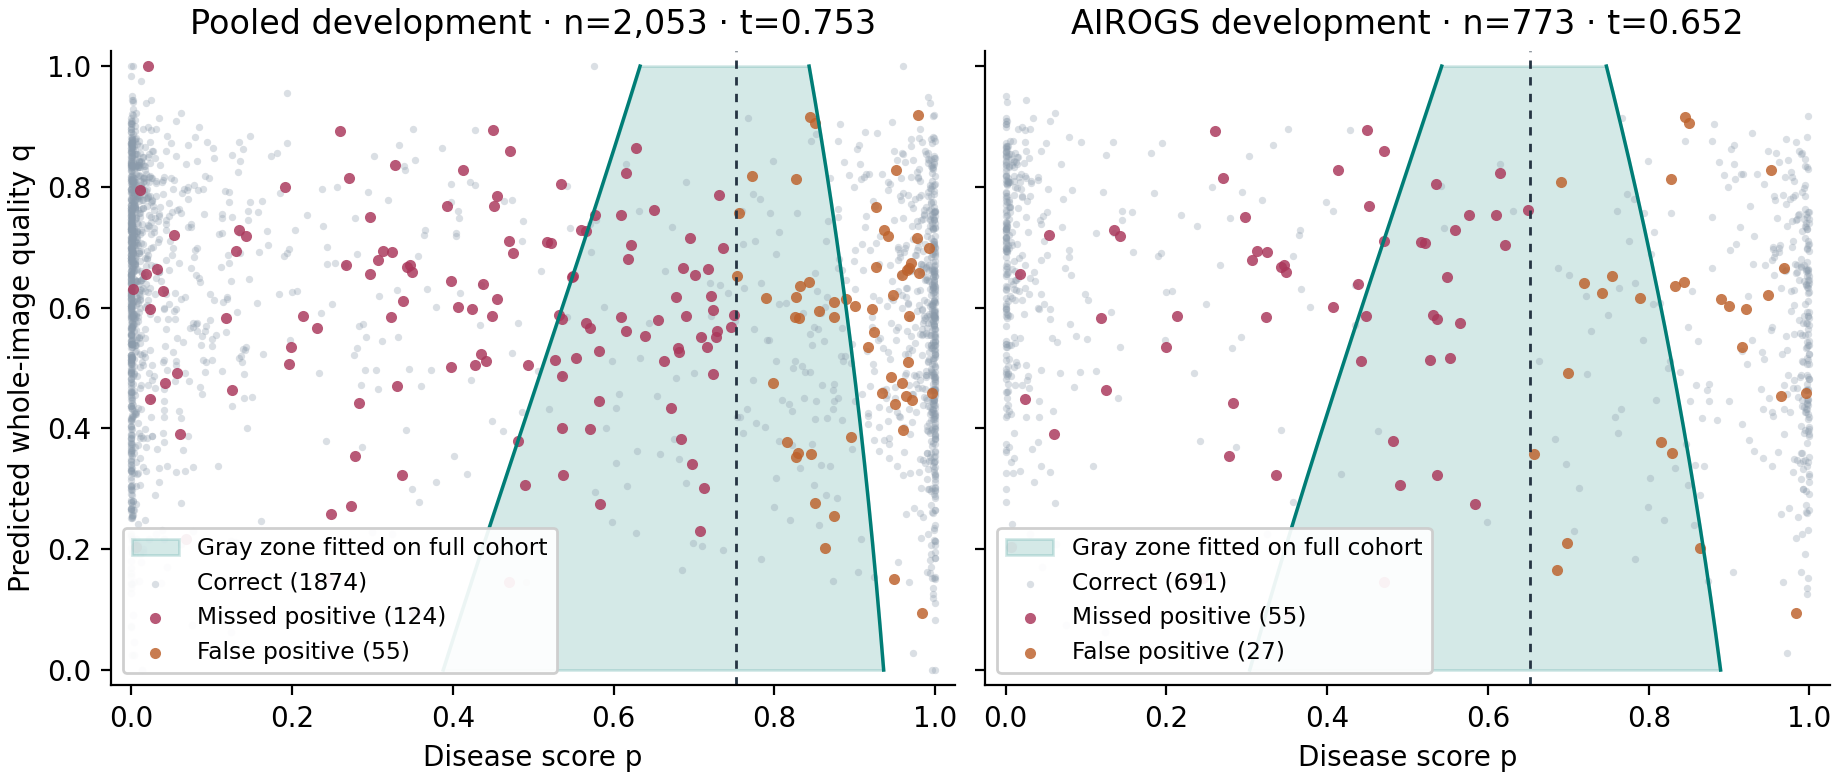
\includegraphics[width=0.98\linewidth,height=\textheight,keepaspectratio,alt={Figure 1. Correct classifications, misses, and false positives in the p--q plane. The dashed line is the disease threshold.}]{gray-zone-map.en.png}
\caption{Figure 1. Correct classifications, misses, and false positives
in the p--q plane. The dashed line is the disease threshold.}
\end{figure}

In pooled development, lowering \(q\) from 1 to 0 widens the eligible
\(p\) interval from 0.633--0.843 to 0.388--0.936. Even at \(q=0\), 46 of
the 124 original misses have disease scores too low to enter the
candidate gray zone. The corresponding AIROGS count is 17 of 55. This
limit matters when designing a separate route for severe defocus or
underexposure.

\begin{figure}
\centering
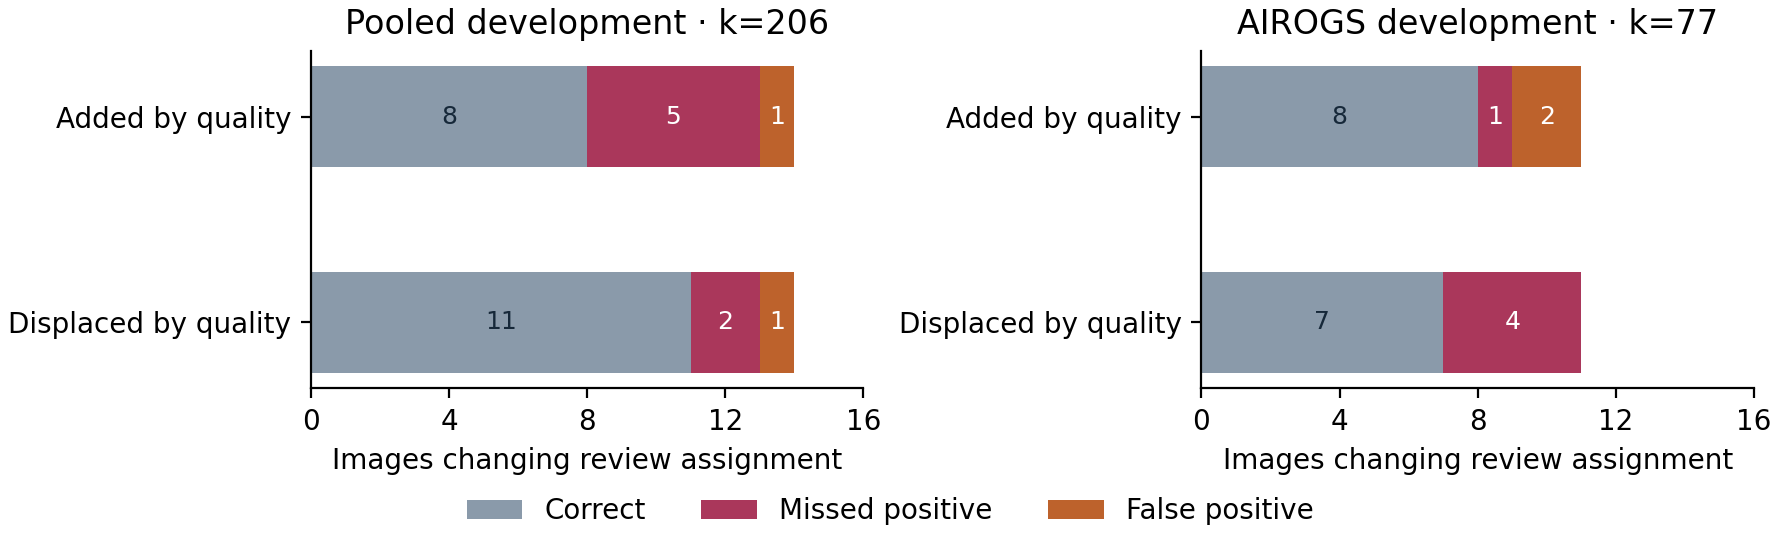
\includegraphics[width=0.98\linewidth,height=\textheight,keepaspectratio,alt={Figure 2. Images added to and displaced from review at the same workload. Color shows A's original classification outcome.}]{review-swaps.en.png}
\caption{Figure 2. Images added to and displaced from review at the same
workload. Color shows A's original classification outcome.}
\end{figure}

The pooled review lists share 192 of their 206 images. Quality adds five
missed positives and one false positive, while displacing two missed
positives and one false positive. AIROGS lists share 66 of 77. Quality
adds one missed positive and two false positives while displacing four
missed positives. These swaps account for the opposite changes in
misses.

\newpage

\subsection{Workload and source}\label{workload-and-source}

\begin{figure}
\centering
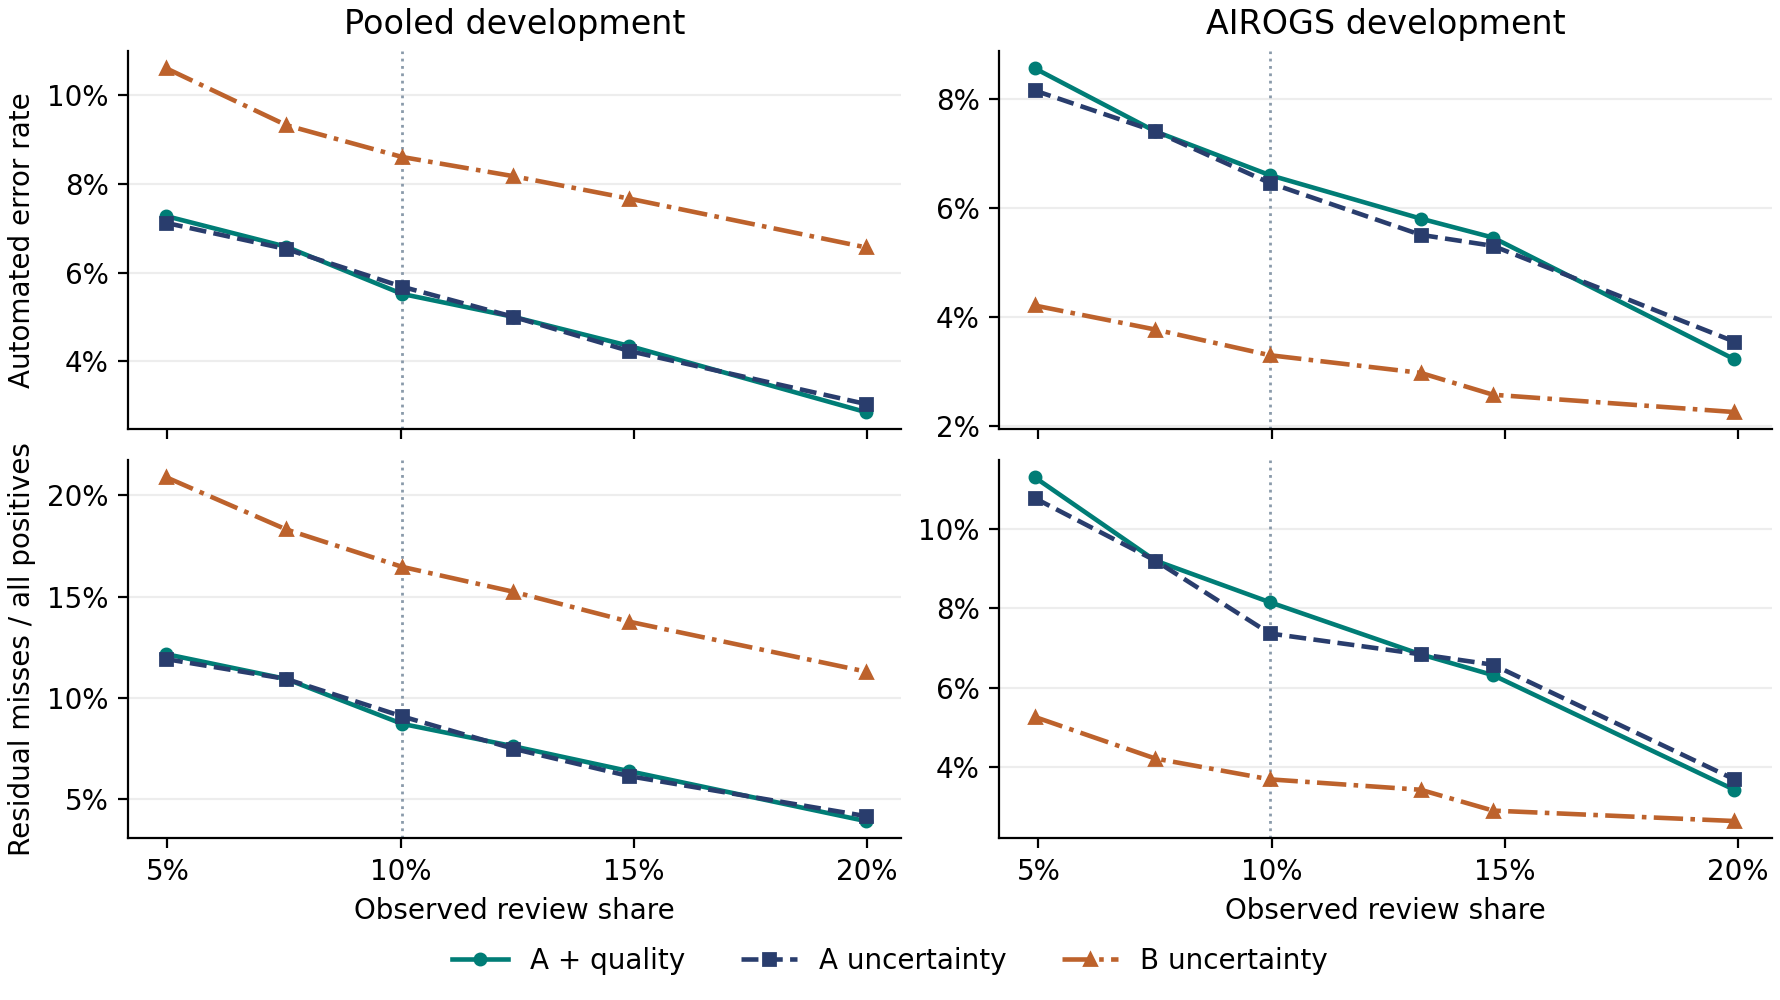
\includegraphics[width=0.92\linewidth,height=\textheight,keepaspectratio,alt={Figure 3. Observed review workload, automated error rate, and remaining misses across six development targets. All methods review the same count at each point.}]{review-workload.en.png}
\caption{Figure 3. Observed review workload, automated error rate, and
remaining misses across six development targets. All methods review the
same count at each point.}
\end{figure}

Across six review targets from 5\% to 20\%, quality changed the
remaining error count relative to A uncertainty by −3 to +3 pooled and
−2 to +3 on AIROGS. At about 10\% review, quality weights of 0.5, 1, and
2 changed pooled errors by −2, −3, and +1. On AIROGS they changed errors
by +1, +1, and +2 and increased misses by two, three, and four. The
weight sweep assesses sensitivity.

\begin{figure}
\centering
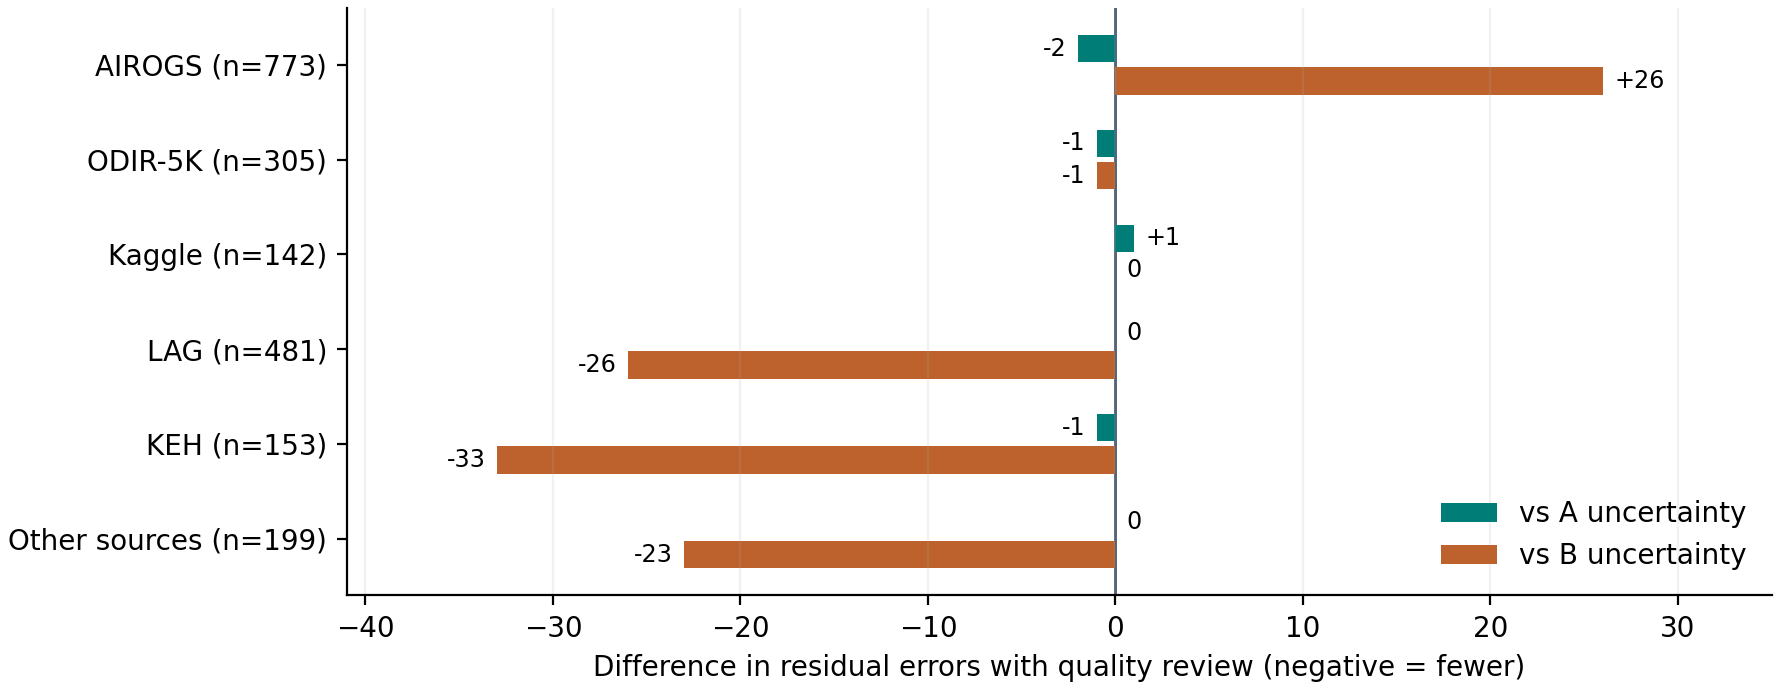
\includegraphics[width=0.9\linewidth,height=\textheight,keepaspectratio,alt={Figure 4. Changes in residual errors by source under the pooled operating point. The pooled policies determine the workload within each source.}]{review-by-source.en.png}
\caption{Figure 4. Changes in residual errors by source under the pooled
operating point. The pooled policies determine the workload within each
source.}
\end{figure}

On pooled data, A with quality left 57 fewer errors than B. A
uncertainty alone left 54 fewer. LAG and KEH contributed a combined −59,
while AIROGS contributed +26. The historical B did not train on LAG or
KEH. With AIROGS-only calibration, B left fewer errors and fewer misses
at all six operating points. This comparison reflects the classifiers,
their training data, and their review policies.

\newpage

\subsection{Candidate cutoffs and independent
test}\label{candidate-cutoffs-and-independent-test}

{\def\LTcaptype{none} % do not increment counter
\begin{longtable}[]{@{}
  >{\raggedright\arraybackslash}p{(\linewidth - 8\tabcolsep) * \real{0.1579}}
  >{\raggedleft\arraybackslash}p{(\linewidth - 8\tabcolsep) * \real{0.2105}}
  >{\raggedleft\arraybackslash}p{(\linewidth - 8\tabcolsep) * \real{0.2105}}
  >{\raggedleft\arraybackslash}p{(\linewidth - 8\tabcolsep) * \real{0.2105}}
  >{\raggedleft\arraybackslash}p{(\linewidth - 8\tabcolsep) * \real{0.2105}}@{}}
\toprule\noalign{}
\begin{minipage}[b]{\linewidth}\raggedright
Candidate cohort
\end{minipage} & \begin{minipage}[b]{\linewidth}\raggedleft
A disease cutoff
\end{minipage} & \begin{minipage}[b]{\linewidth}\raggedleft
B disease cutoff
\end{minipage} & \begin{minipage}[b]{\linewidth}\raggedleft
Gray-zone cutoff \(s\)
\end{minipage} & \begin{minipage}[b]{\linewidth}\raggedleft
Validation / development
\end{minipage} \\
\midrule\noalign{}
\endhead
\bottomrule\noalign{}
\endlastfoot
Pooled & 0.752843 & 0.581313 & −0.568675 & 2,046 / 2,053 \\
AIROGS & 0.651953 & 0.815315 & −0.457006 & 767 / 773 \\
\end{longtable}
}

Each candidate cutoff is taken from the upper tail of review scores on
its full development cohort, targeting about 10\%. Before independent
evaluation, define the primary cohort and fix its thresholds, weight,
checkpoints, preprocessing, and tie-breaking rule. The fixed boundary
then produces the actual test workload \(k\), and both controls review
\(k\) photographs in that cohort. AIROGS labels describe whether a case
meets the referral criterion.
\href{https://airogs.grand-challenge.org/data-and-challenge/}{Official
AIROGS evaluation}

{\def\LTcaptype{none} % do not increment counter
\begin{longtable}[]{@{}
  >{\raggedright\arraybackslash}p{(\linewidth - 8\tabcolsep) * \real{0.1579}}
  >{\raggedleft\arraybackslash}p{(\linewidth - 8\tabcolsep) * \real{0.2105}}
  >{\raggedleft\arraybackslash}p{(\linewidth - 8\tabcolsep) * \real{0.2105}}
  >{\raggedleft\arraybackslash}p{(\linewidth - 8\tabcolsep) * \real{0.2105}}
  >{\raggedleft\arraybackslash}p{(\linewidth - 8\tabcolsep) * \real{0.2105}}@{}}
\toprule\noalign{}
\begin{minipage}[b]{\linewidth}\raggedright
Reserved cohort
\end{minipage} & \begin{minipage}[b]{\linewidth}\raggedleft
Images
\end{minipage} & \begin{minipage}[b]{\linewidth}\raggedleft
Positives
\end{minipage} & \begin{minipage}[b]{\linewidth}\raggedleft
Linked groups
\end{minipage} & \begin{minipage}[b]{\linewidth}\raggedleft
Recorded poor-quality positive / negative
\end{minipage} \\
\midrule\noalign{}
\endhead
\bottomrule\noalign{}
\endlastfoot
Internal and new holdouts & 3,470 & 1,292 & 3,045 & 50 / 18 \\
AIROGS within those holdouts & 770 & 385 & 770 & 0 / 0 \\
ACRIMA external & 705 & 396 & 705 & 0 / 0 \\
HYGD external & 737 & 540 & 283 & 0 / 0 \\
\end{longtable}
}

The audit used manifest metadata only. The reserved images show no
recorded group or file SHA-256 overlap with A's training, model
validation, or rule development, no original group or file hash overlap
with B's training or validation, and no hash overlap with joint quality
training or validation. These checks cover recorded links and identical
files. FIVES contributes all 18 poor-quality negatives and 41 positives
using its official quality dimensions. MSHF adds nine positives rated
poor overall. A zero means that no cases were recorded by these
definitions.

\textbf{The proposal needs an explicit route for positive calls.} Page 4
depicts about 10\% manual review, a retake branch, and automated
classification for high-confidence normals. The current gray zone leaves
634 A-positive calls in the pooled automated branch and 306 on AIROGS.
Sending them all to manual review would raise workloads to 840/2,053
(40.9\%) and 383/773 (49.5\%). These figures use the current development
cohorts. The evaluation should specify direct referral, manual grading,
and disposition after a retake.

The current evidence supports progress on disease ranking in some
sources and reproducible gray-zone triage. The incremental value of
whole-image quality still needs independent testing. A retake evaluation
requires first and repeat photographs of the same eye with a reference
diagnosis. The development set has 12 human-graded poor-quality
positives and zero such negatives, and retake recovery remains
unmeasured.

\href{gray-zone-results.json}{Full operating points, candidate cutoffs,
and data hashes} ·
\href{../../../tools/audit_gray_zone_20261118.py}{Analysis script} ·
\href{../../../tools/plot_gray_zone_20261118.py}{Plot script}

\end{document}
